\section{Superposition}
\label{sec:superposition}

The previous section highlighted a limitation of interpretable directions.
Only a limited number of concepts can be represented by a linear direction, and these directions are often entangled with multiple semantic concepts.
To account for this, an extension of the \ConceptHypothesisName has been proposed under the name \SuperpositionHypothesisName, formalized in Hypothesis~\ref{hyp:superposition} \cite{elhage2022superposition}.

\begin{hypothesis}{Superposition Hypothesis}{superposition}
Concepts are preferentially represented by distinct linear directions in \gls{ls}.
When the number of concepts exceeds the available dimensions, multiple concepts are encoded in superposition within the same directions.
\end{hypothesis}

According to this hypothesis, in an unconstrained \gls{ls}, each concept is represented in its own independent linear direction.
The idealized non-superposed \gls{lr} can be mathematically expressed as follows:
\[
\latentRepresentation = \sum_{i=1}^{n} \alpha_i \mathbf{v}_i,
\qquad
\forall i \neq j,\quad \mathbf{v}_i^\top \mathbf{v}_j \approx 0,
\qquad
\|\boldsymbol{\alpha}\|_0 \ll n,
\]

where:
\begin{itemize}
    \item $\latentRepresentation$ denotes a \gls{lr},
    \item $n$ is the total number of concepts,
    \item $\mathbf{v}_i$ represents the direction associated with concept $c_i$,
    \item $\alpha_i$ corresponds to the activation strength of concept $c_i$ in the \gls{lr} $\latentRepresentation$,
    \item $\mathbf{v}_i^\top \mathbf{v}_j \approx 0$ indicates that concept directions are approximately orthogonal, meaning each concept independently controls a single factor of variation,
    \item $\|\boldsymbol{\alpha}\|_0 \ll n$ indicates that only a small fraction of concepts are active for a given \gls{lr}.
\end{itemize}

However, \gls{nn} operate in finite-dimensional spaces, so when the number of concepts exceeds the available dimensions, such a one-to-one correspondence becomes impractical.
The network must therefore reuse its representational dimensions, allowing multiple concepts to be encoded using the same directions.
This shared encoding is referred to as superposition \cite{bricken2023monosemanticity}.
This phenomenon becomes an obstacle for any method that attempts to analyze \gls{lr} directly in the original activation space.

Building on this observation, several works based on the \SuperpositionHypothesisName have developed methods that aim to recover less superposed \gls{lr}.
A common approach is to map \gls{ls} into a higher-dimensional space while imposing additional constraints that encourage individual concepts to be represented separately.
This transformation is illustrated in Figure~\ref{fig:dense_to_sparse_sae}, while \gls{lr} are entangled in the initial \gls{ls}, the sparse representation aligns each concept with a dedicated feature axis.

\providecommand{\lsePanelWidth}{6cm}
\newlength{\saePanelWd}
\newlength{\saePanelHt}
\newlength{\saePanelGap}

% Lengths must be set BEFORE \resizebox so pgfplots sees non-zero values.
\setlength{\saePanelWd}{\lsePanelWidth}
\pgfmathsetlength{\saePanelHt} {\saePanelWd * 5 / 6}
\pgfmathsetlength{\saePanelGap}{\saePanelWd * 0.9}

\begin{figure}[t]
\centering

% ================================================================
%  latent_space_shared.tex
%  Couleurs, macros et styles partagés par toutes les figures
%  latent_space_*.tex
%  Usage : % ================================================================
%  latent_space_shared.tex
%  Couleurs, macros et styles partagés par toutes les figures
%  latent_space_*.tex
%  Usage : \input{figures/latent_space/latent_space_shared.tex}
% ================================================================

% ----------------------------------------------------------------
% Couleurs des clusters
% ----------------------------------------------------------------
\colorlet{colorA}{blue!70!cyan}
\colorlet{colorB}{orange}
\colorlet{colorC}{green!60!black}

% Couleurs de directions (latent_space_directions.tex)
\colorlet{colorDirBA}{violet}
\colorlet{colorDirBC}{red!70!black}

% ----------------------------------------------------------------
% Macros de dessin
% ----------------------------------------------------------------
\input{figures/latent_space/plot_points.tex}
\input{figures/latent_space/plot_ellipse.tex}
\input{figures/latent_space/plot_probe.tex}
\input{figures/latent_space/plot_direction.tex}

% ----------------------------------------------------------------
% Styles d'axe partagés
% ----------------------------------------------------------------
\pgfplotsset{
  % Axe standard (clustering, probing, directions)
  latent axis/.style={
    width=11cm,
    height=10cm,
    xmin=-7, xmax=8,
    ymin=-7, ymax=5.5,
    axis x line=bottom,
    axis y line=left,
    axis line style={
      -{Stealth[length=8pt, width=6pt]},
      thick
    },
    ticks=none,
    xlabel={},
    ylabel={},
    clip=true,
  },
  % Variante panneau carré (latent_space_sparse_autoencoders.tex)
  latent panel/.style={
    latent axis,
    width=9cm,
    height=9cm,
  },
  % Variante petit panneau (latent_space_embeddings.tex)
  % N.B. width/height sont passés explicitement par chaque fichier
  % via width=\lsePanelWd, height=\lsePanelHt dans l'axe.
  latent embed/.style={
    latent axis,
    every axis plot/.append style={forget plot},
  },
}

% ================================================================

% ----------------------------------------------------------------
% Couleurs des clusters
% ----------------------------------------------------------------
\colorlet{colorA}{blue!70!cyan}
\colorlet{colorB}{orange}
\colorlet{colorC}{green!60!black}

% Couleurs de directions (latent_space_directions.tex)
\colorlet{colorDirBA}{violet}
\colorlet{colorDirBC}{red!70!black}

% ----------------------------------------------------------------
% Macros de dessin
% ----------------------------------------------------------------
% ================================================================
%  \plotPoints — Reusable macro to render a point cloud from file
%
%  Usage:
%    \plotPoints[color=<c>, size=<s>, opacity=<o>]{<file.data>}
%
%  Arguments (all optional, defaults shown below):
%    color   : fill & stroke color of the markers  (default: black)
%    size    : marker radius                        (default: 2pt)
%    opacity : fill opacity [0..1]                  (default: 0.85)
%
%  Positional (mandatory):
%    #1 : path to a whitespace-separated x y data file
%         (lines starting with % are treated as comments)
%
%  Example:
%    \plotPoints[color=blue!70!cyan, size=3pt]{data/cluster_a.data}
% ================================================================
\pgfkeys{
  /plotPoints/.is family, /plotPoints,
  % --- defaults ---
  color/.initial   = black,
  size/.initial    = 2pt,
  opacity/.initial = 0.85,
}

\newcommand{\plotPoints}[2][]{%
  \pgfkeys{/plotPoints, #1}%                     % apply user overrides
  \pgfkeysgetvalue{/plotPoints/color}  {\ppColor}%
  \pgfkeysgetvalue{/plotPoints/size}   {\ppSize}%
  \pgfkeysgetvalue{/plotPoints/opacity}{\ppOpacity}%
  \addplot[
    only marks,
    mark        = *,
    mark size   = \ppSize,
    mark options= {fill=\ppColor, draw=\ppColor, fill opacity=\ppOpacity},
  ] file {#2};%
}
% ================================================================
%  \plotEllipse — Companion macro to draw a confidence ellipse
%
%  Usage:
%    \plotEllipse[color=<c>, width=<w>]
%                {<cx>}{<cy>}{<angle>}{<rx>}{<ry>}
%
%  Arguments (all optional):
%    color : stroke color  (default: black)
%    width : line width    (default: very thick)
%
%  Positional (mandatory):
%    {cx}    : ellipse center x  (axis coordinates)
%    {cy}    : ellipse center y  (axis coordinates)
%    {angle} : counter-clockwise rotation in degrees
%    {rx}    : horizontal semi-axis (cm)
%    {ry}    : vertical   semi-axis (cm)
%
%  Example:
%    \plotEllipse[color=orange]{-3}{1.5}{15}{2.3}{1.2}
% ================================================================
\pgfkeys{
  /plotEllipse/.is family, /plotEllipse,
  color/.initial = black,
  width/.initial = very thick,
}

\newcommand{\plotEllipse}[6][]{%
  \pgfkeys{/plotEllipse, #1}%
  \pgfkeysgetvalue{/plotEllipse/color}{\peColor}%
  \pgfkeysgetvalue{/plotEllipse/width}{\peWidth}%
  \draw[\peColor, \peWidth, rotate around={#4:(#2,#3)}]
    (#2,#3) ellipse (#5cm and #6cm);%
}
% ================================================================
%  plot_probe.tex — Linear probing decision boundary
%
%  \plotProbe[<options>]{<slope>}{<intercept>}
%
%  Draws  y = slope*x + intercept  clipped to the axis bounds.
%
%  Options (all optional):
%    color : line color   (default: black)
%    style : dash pattern (default: dashed)
%    width : line width   (default: thick)
%
%  WHY \edef ON THE WHOLE CALL: same deferred-rendering issue as
%  plot_points.tex — pgfplots evaluates ALL \addplot options at
%  \end{axis}, not at call time, so macro values must be baked in.
%
%  Example:
%    \plotProbe[color=colorA]{1}{3}
% ================================================================
\pgfkeys{
  /plotprobe/.is family, /plotprobe,
  color/.initial = black,
  style/.initial = dashed,
  width/.initial = thick,
}

\newcommand{\plotProbe}[3][]{%
  \pgfkeys{/plotprobe, #1}%
  \pgfkeysgetvalue{/plotprobe/color}{\prColor}%
  \pgfkeysgetvalue{/plotprobe/style}{\prStyle}%
  \pgfkeysgetvalue{/plotprobe/width}{\prWidth}%
  \edef\prDoPlot{%
    \noexpand\addplot[%
      domain=-7:8, samples=2,%
      \prStyle, \prWidth, color=\prColor, forget plot%
    ] {#2 * x + (#3)};%
  }%
  \prDoPlot
}

% ================================================================
%  plot_direction.tex — Interpretable direction vector
%
%  \plotDirection[<options>]{<x1>}{<y1>}{<x2>}{<y2>}
%
%  Draws a thick arrow from (x1,y1) to (x2,y2) in axis coordinates.
%  Must be called OUTSIDE the \addplot system, directly inside axis.
%
%  Options (all optional):
%    color   : arrow color   (default: black)
%    width   : line width    (default: very thick)
%    shorten : shorten tip   (default: 4pt)
%
%  Example:
%    \plotDirection[color=colorA]{-2.5}{-4}{-3}{1.5}
% ================================================================
\pgfkeys{
  /plotdirection/.is family, /plotdirection,
  color/.initial   = black,
  width/.initial   = very thick,
  shorten/.initial = 4pt,
}

\newcommand{\plotDirection}[6][]{%
  \pgfkeys{/plotdirection, #1}%
  \pgfkeysgetvalue{/plotdirection/color}  {\pdColor}%
  \pgfkeysgetvalue{/plotdirection/width}  {\pdWidth}%
  \pgfkeysgetvalue{/plotdirection/shorten}{\pdShorten}%
  \draw[\pdColor, \pdWidth, -Stealth,
        shorten >=\pdShorten, shorten <=\pdShorten]
    (axis cs:#2,#3) -- (axis cs:#4,#5);%
}


% ----------------------------------------------------------------
% Styles d'axe partagés
% ----------------------------------------------------------------
\pgfplotsset{
  % Axe standard (clustering, probing, directions)
  latent axis/.style={
    width=11cm,
    height=10cm,
    xmin=-7, xmax=8,
    ymin=-7, ymax=5.5,
    axis x line=bottom,
    axis y line=left,
    axis line style={
      -{Stealth[length=8pt, width=6pt]},
      thick
    },
    ticks=none,
    xlabel={},
    ylabel={},
    clip=true,
  },
  % Variante panneau carré (latent_space_sparse_autoencoders.tex)
  latent panel/.style={
    latent axis,
    width=9cm,
    height=9cm,
  },
  % Variante petit panneau (latent_space_embeddings.tex)
  % N.B. width/height sont passés explicitement par chaque fichier
  % via width=\lsePanelWd, height=\lsePanelHt dans l'axe.
  latent embed/.style={
    latent axis,
    every axis plot/.append style={forget plot},
  },
}


\resizebox{1\textwidth}{!}{
\begin{tikzpicture}

  % ================================================================
  % LEFT PANEL — Dense latent space
  % ================================================================
  \begin{scope}[xshift=0pt]
  \begin{axis}[
    name=axisLeft,
    latent embed,
    width=\saePanelWd,
    height=\saePanelHt,
    xmin=-7, xmax=8,
    ymin=-7, ymax=5.5,
  ]
    \plotPoints[color=colorA]{figures/latent_space/cluster_a.data}
    \plotPoints[color=colorB]{figures/latent_space/cluster_b.data}
    \plotPoints[color=colorC]{figures/latent_space/cluster_c.data}
  \end{axis}
  \node[anchor=north, yshift=-6pt] at (axisLeft.south)
    {\textbf{(a)} Dense latent space};
  \end{scope}

  % ================================================================
  % RIGHT PANEL — Sparse SAE space
  % ================================================================
  \begin{scope}[xshift=\saePanelGap]
  \begin{axis}[
    name=axisRight,
    width=\saePanelWd,
    height=\saePanelHt,
    xmin=-8.5, xmax=8.5,
    ymin=-6,   ymax=9,
    axis lines=none,
    ticks=none,
    clip=true,
  ]

    \draw[colorA, thick, -{Stealth[length=7pt,width=5pt]}]
      (axis cs:0,0) -- (axis cs:0,7);
    \node[colorA, font=\small\bfseries, above] at (axis cs:0,7.3)
      {Feature $A$};

    \draw[colorB, thick, -{Stealth[length=7pt,width=5pt]}]
      (axis cs:0,0) -- (axis cs:-6.062,-3.5);
    \node[colorB, font=\small\bfseries, below left] at (axis cs:-6.062,-3.8)
      {Feature $B$};

    \draw[colorC, thick, -{Stealth[length=7pt,width=5pt]}]
      (axis cs:0,0) -- (axis cs:6.062,-3.5);
    \node[colorC, font=\small\bfseries, below right] at (axis cs:6.062,-3.8)
      {Feature $C$};

    \plotPoints[color=colorA]{figures/latent_space/sae_right_a.data}
    \plotPoints[color=colorB]{figures/latent_space/sae_right_b.data}
    \plotPoints[color=colorC]{figures/latent_space/sae_right_c.data}

  \end{axis}
  \node[anchor=north, yshift=-6pt] at (axisRight.south)
    {\textbf{(b)} Sparse SAE space};
  \end{scope}

\end{tikzpicture}
}

\caption{
  Transformation from a dense latent space to a sparse SAE-style representation.
  On the left \textbf{(a)}, embeddings are entangled in the initial latent space.
  On the right \textbf{(b)}, the sparse representation aligns each concept with a dedicated feature axis.
}
\label{fig:dense_to_sparse_sae}
\end{figure}


\gls{sae} provide a practical implementation of this approach and can be defined as follows:
\[
z = f_{\text{enc}}(\latentRepresentation), \quad \hat{\latentRepresentation} = f_{\text{dec}}(z)
\]
\[
\mathcal{L}_{\text{auto}} = \gamma \|\latentRepresentation - \hat{\latentRepresentation}\|_2^2 + \lambda \|z\|_1
\]

where:
\begin{itemize}
    \item $f_{\text{enc}}(\latentRepresentation)$ is the encoding function that projects the original \gls{lr} $\latentRepresentation$ into a higher-dimensional sparse space,
    \item $f_{\text{dec}}(z)$ is the decoding function that reconstructs the original \gls{lr} from the sparse code,
    \item $z \in \mathcal{Z}$ is the sparse representation of $\latentRepresentation$, with $\dim(z) \gg \dim(\latentRepresentation)$,
    \item $\hat{\latentRepresentation}$ is the reconstructed \gls{lr},
    \item $\|\latentRepresentation - \hat{\latentRepresentation}\|_2^2$ is the reconstruction loss ensuring that the original \gls{lr} can be faithfully recovered,
    \item $\|z\|_1$ is the sparsity regularization term that encourages most components of $z$ to be zero,
    \item $\gamma, \lambda$ are weighting coefficients controlling the trade-off between reconstruction fidelity and sparsity.
\end{itemize}

The parameters of these projection functions $f_{\text{enc}}$ and $f_{\text{dec}}$ are learned by minimizing $\mathcal{L}_{\text{auto}}$ using \gls{sgd}.
Under this formulation, each dimension of $\mathcal{Z}$ is interpreted as a dedicated concept direction.

In practice, both $f_{\text{enc}}$ and $f_{\text{dec}}$ are implemented as linear projections between the original \gls{ls} and the high-dimensional space $\mathcal{Z}$. This choice is motivated by the same principle underlying probing methods. The transformation applied to the \gls{lr} should remain as simple as possible.
Using more expressive projection functions could introduce additional structures into the transformed \gls{lr}. In this case, it would become difficult to determine whether an observed concept was already encoded in the model's \gls{lr}, or whether it was introduced by the projection itself. Restricting $f_{\text{enc}}$ and $f_{\text{dec}}$ to linear projections therefore helps ensure that the concepts identified in $\mathcal{Z}$ can be attributed to the original \gls{lr}, rather than to the transformation used to analyze it.

The method proves to be powerful when successfully applied to language models \cite{templeton2024scaling}.
In these applications, \gls{sae} are used to desuperpose the \gls{lr} of \gls{llm}.
Once this \gls{lr} is obtained, it has been shown that many concept vectors exhibit semantic properties.
A example is the Golden Gate Bridge concept direction, illustrated in Figure~\ref{fig:sparse_autoencoder_illustration}, which activates systematically whenever the input text or image refers to the Golden Gate Bridge, regardless of the language or modality.
This demonstrates that the learned concept is not tied to a specific surface form but captures a deeper semantic abstraction shared across modalities.

\begin{figure}[t]
    \centering
    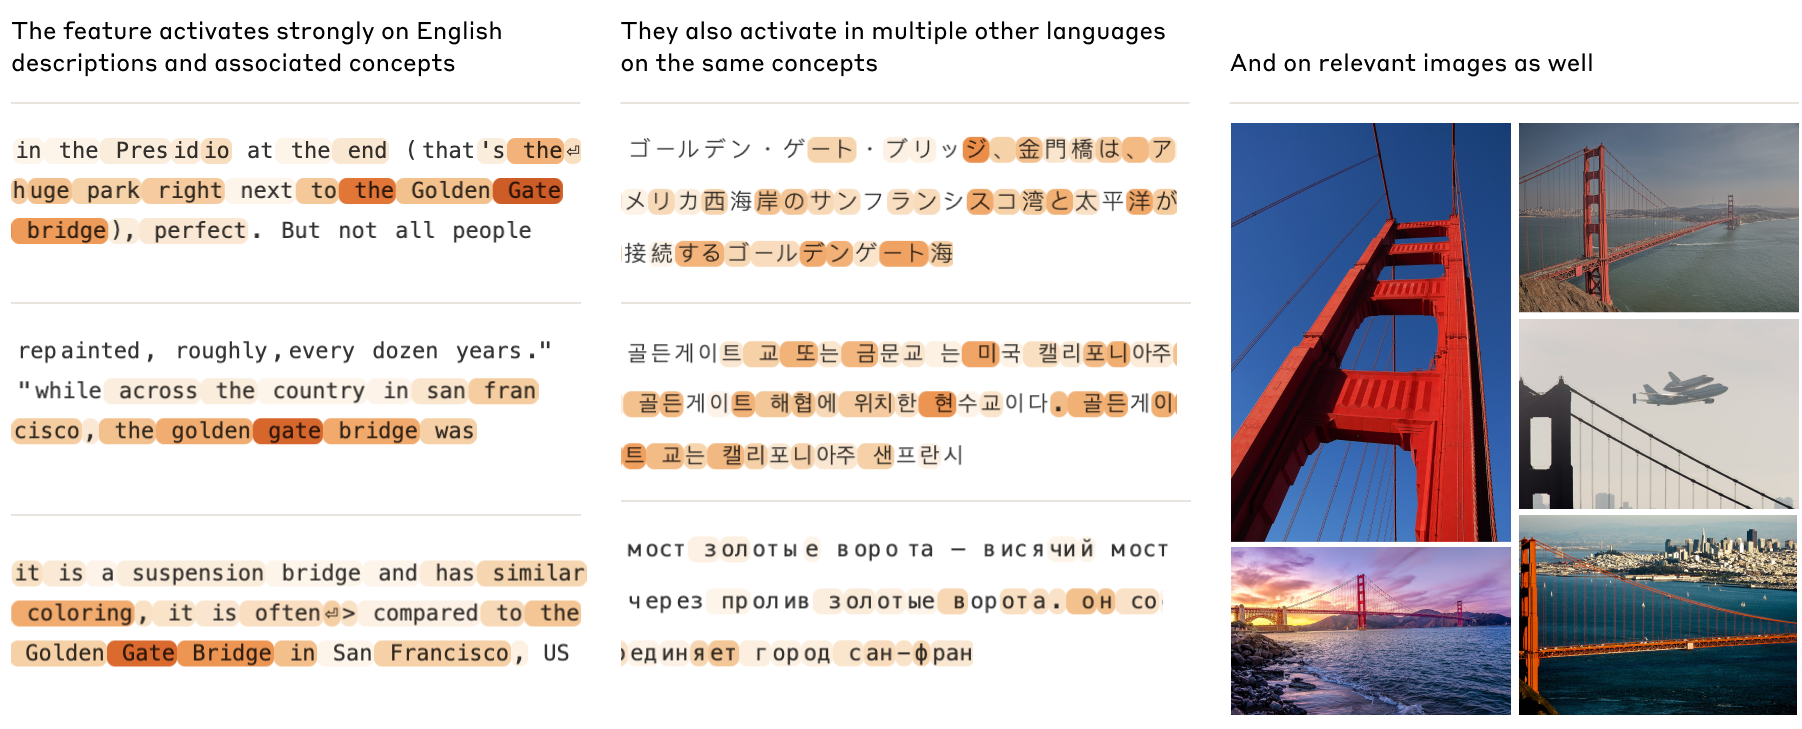
\includegraphics[width=0.85\textwidth]
        {figures/latent_space/sparse_autoencoder_illustration.png}
    \caption{
        A concept direction corresponding to the Golden Gate Bridge, discovered
        by a sparse autoencoder applied to a large language model
        \cite{templeton2024scaling}.
    }
    \label{fig:sparse_autoencoder_illustration}
\end{figure}

\gls{sae} also provide a way to intervene directly on the \gls{lr} learned by the model.
A concept can be artificially activated by modifying its corresponding feature in the sparse representation $z$, even when the input contains no reference to it.
The modified \gls{lr} is then projected back into the original activation space, after which the model proceeds with standard next-token generation from $\latentRepresentation^{*}$:
\[
\latentRepresentation^{*} = f_{\text{dec}}(z^*), \quad \text{where} \quad z^* = z + \delta \, e_i,
\]

where:
\begin{itemize}
    \item $z$ is the original sparse representation of the input,
    \item $z^*$ is the modified sparse representation,
    \item $e_i$ is the basis vector of $\mathcal{Z}$ associated with the target concept direction,
    \item $\delta$ controls the strength of the artificial activation,
    \item $\latentRepresentation^{*}$ is the resulting edited \gls{lr} in the original activation space.
\end{itemize}

With this method, a reference to the Golden Gate Bridge can be injected into the \gls{llm}'s internal representation.
This causes the model's output to shift toward discussing the Golden Gate Bridge, even when the prompt contains no reference to it.
This provides evidence that the learned feature plays a causal role in the model's behavior.
Such interventions enable control over specific model behaviors through \gls{ls} editing.

Despite their empirical success, \SuperpositionHypothesisName exhibit several important limitations that question their assumptions. 
These limitations can be summarized as follows:
\begin{itemize}
    \item \textbf{Instability of the decomposition.}
    Repeating the \gls{sae} training process multiple times on the same model does not yield the same decomposition of the \gls{ls}.
    Different runs produce different concept directions in $\mathcal{Z}$, even when achieving comparable reconstruction performance, which raises questions about the reliability of the discovered \gls{cs}.

    \item \textbf{Lack of semantic coverage.}
    In the high-dimensional space $\mathcal{Z}$, a large fraction of dimensions do not correspond to any interpretable semantic concept.
    This abundance of non-semantic directions raises questions about whether the decomposition truly reflects the model’s \gls{cs}.

    \item \textbf{Sparsity--semantics trade-off.}
    Increasing the sparsity coefficient $\lambda$ beyond a certain threshold degrades the semantic quality of the learned features \cite{tanhPenaltyDictionaryLearning}.
    Suggesting that enforcing excessive sparsity comes at the cost of interpretability.

    \item \textbf{Failure of scaling to remove superposition.}
    Under the \SuperpositionHypothesisName, increasing the dimensionality of the \gls{ls} should reduce superposition.
    However, this is not observed in practice.
    Even in very high-dimensional \gls{ls}, representations remain superposed, indicating that scaling alone does not resolve the entanglement.
\end{itemize}

These limitations suggest that \SuperpositionHypothesisName, while powerful, do not fully resolve the problem of \gls{cs}.
Convincing empirical results do not necessarily validate the underlying theoretical assumptions.

So far, every method described, whether based on probing, interpretable directions, or superposition, relies on a common assumption.
The \gls{cs} can be recovered from \gls{lr} through a linear decomposition.
This assumption has enabled substantial progress in understanding neural representations, but it also imposes a strong constraint on how concepts are expected to be represented.
The following section examines clustering as an alternative approach that does not rely on this assumption.